%%%%%%%%%%%%%%%%%%%%%%%%%%%%%%%%%%%%%%%%%%%%%%%%%%%%%%%%%%%%%%%%%%%%%%%%
%    INSTITUTE OF PHYSICS PUBLISHING                                   %
%                                                                      %
%   `Preparing an article for publication in an Institute of Physics   %
%    Publishing journal using LaTeX'                                   %
%                                                                      %
%    LaTeX source code `ioplau2e.tex' used to generate `author         %
%    guidelines', the documentation explaining and demonstrating use   %
%    of the Institute of Physics Publishing LaTeX preprint files       %
%    `iopart.cls, iopart12.clo and iopart10.clo'.                      %
%                                                                      %
%    `ioplau2e.tex' itself uses LaTeX with `iopart.cls'                %
%                                                                      %
%%%%%%%%%%%%%%%%%%%%%%%%%%%%%%%%%%
%
%
% First we have a character check
%
% ! exclamation mark    " double quote  
% # hash                ` opening quote (grave)
% & ampersand           ' closing quote (acute)
% $ dollar              % percent       
% ( open parenthesis    ) close paren.  
% - hyphen              = equals sign
% | vertical bar        ~ tilde         
% @ at sign             _ underscore
% { open curly brace    } close curly   
% [ open square         ] close square bracket
% + plus sign           ; semi-colon    
% * asterisk            : colon
% < open angle bracket  > close angle   
% , comma               . full stop
% ? question mark       / forward slash 
% \ backslash           ^ circumflex
%
% ABCDEFGHIJKLMNOPQRSTUVWXYZ 
% abcdefghijklmnopqrstuvwxyz 
% 1234567890
%
%%%%%%%%%%%%%%%%%%%%%%%%%%%%%%%%%%%%%%%%%%%%%%%%%%%%%%%%%%%%%%%%%%%
%

%AIP Reprint Class%%%%%%%%%%%%%%%%%%%%%%%%%%%%%%%%%%%%%%%%%%%%%%%%%%%%%%%%%%%%%%%%%%%%%%%%%%%%%
\documentclass[aip,prl,amsmath,amssymb,reprint,superscriptaddress]{revtex4-1} %preprint version
\usepackage{graphicx}% Include figure files
\usepackage{dcolumn}% Align table columns on decimal point
\usepackage{bm}% bold math
\usepackage{epstopdf}

    \renewcommand{\topfraction}{0.9}    % max fraction of floats at top
    \renewcommand{\bottomfraction}{0.8}    % max fraction of floats at bottom
    \setcounter{topnumber}{2}
    \setcounter{bottomnumber}{2}
    \setcounter{totalnumber}{4}     % 2 may work better
    \setcounter{dbltopnumber}{2}    % for 2-column pages
    \renewcommand{\dbltopfraction}{0.9}    % fit big float above 2-col. text
    \renewcommand{\textfraction}{0.07}    % allow minimal text w. figs
    \renewcommand{\floatpagefraction}{0.7}    % require fuller float pages
    \renewcommand{\dblfloatpagefraction}{0.7}    % require fuller float pages
    \setlength{\abovecaptionskip}{5pt}
    \setlength{\belowcaptionskip}{5pt}
    \setlength{\parskip}{0pt}
    \setlength{\textfloatsep}{5pt} 

%%%%%%%%%%%%%%%%%%%%%%%%%%%%%%%%%%%%%%%%%%%%%%%%%%%%%%%%%%%%%%%%%%%%%%%%%%%%%%%%%%%%%%%%%%%%%%%%%%

%IOP preprint class %%%%%%%%%%%%%%%%%%%%%%%%%%%%%%%%%%%%%%%%%%%%%%%%%%%%%%%%%%%%%%%%%%%%%%%%%%%%%%
%\documentclass[12pt]{iopart}
%\newcommand{\gguide}{{\it Preparing graphics for IOP journals}}
%Uncomment next line if AMS fonts required
%\usepackage{iopams}
%\usepackage{graphicx}
%\usepackage{epstopdf}  
%%%%%%%%%%%%%%%%%%%%%%%%%%%%%%%%%%%%%%%%%%%%%%%%%%%%%%%%%%%%%%%%%%%%%%%%%%%%%%%%%%%%%%%%%%%%%%%%%%
%Slava's inserts %%%%%%%%%%%%%%%%%%%%%%%%%%%%%%%%%%%%%%%%%%%%%%%%%%%%%%%%%%%%%%%%%%%%%%%%%%%%%%
%\usepackage{amsfonts}
%\usepackage{amssymb}

%\newcommand{\ptt}[1]{\frac{\partial#1}{\partial t}}
%\newcommand{\vvec}{\mathbf{v}}
%\newcommand{\Bvec}{\mathbf{B}}
%\newcommand{\Evec}{\mathbf{E}}
%\newcommand{\Jvec}{\mathbf{J}}
%\newcommand{\Avec}{\mathbf{A}}
%%%%%%%%%%%%%%%%%%%%%%%%%%%%%%%%%%%%%%%%%%%%%%%%%%%%%%%%%%%%%%%%%%%%%%%%%%%%%%%%%%%%%%%%%%%%%%%%%%

\begin{document}
\title{Spatial correlations in a turbulent MHD laboratory plasma}

\author{A. Wan}
\affiliation{Swarthmore College, Swarthmore, PA, USA}
\author{D.A. Schaffner}
\affiliation{Swarthmore College, Swarthmore, PA, USA}
\author{V.S. Lukin}
\affiliation{Space Science Division, Naval Research Laboratory, Washington, DC, USA}
\author{W.H. Matthaeus}
\affiliation{Bartol Research Institute and Department of Physics and Astronomy, University of Deleware, Newark, DE, USA}
\author{M.R. Brown}
\affiliation{Swarthmore College, Swarthmore, PA, USA}
\date{\today}
\begin{abstract}
Correlation analysis is used to determine the Taylor microscale and magnetic Reynold's number in a turbulent laboratory MHD plasma.  We find that radial correlation length is shorter for a colliding MHD wind tunnel plasma than for a single plume.  An unambiguous measure of the magnetic Reynolds number is estimated from the Taylor microscale and the correlation scale, then compared to a calculation using the Spitzer resistivity.
\end{abstract}

\maketitle

\section{Introduction}

A useful measure of fully developed turbulence is the spatial correlation function.  For a magnetohydrodynamic (MHD) plasma, the magnetic correlation function can be written
%
\begin{equation}
R(r) =  \langle {\bf b(x) \cdot b(x + r)} \rangle
\label{eq:correlation1}
\end{equation}
%
where {\bf b} is the fluctuating part of a turbulent magnetic field (${\bf B}(x, t) = {\bf B_0 + b}$).  For well-behaved turbulence, the magnetic fluctuations at two points should become uncorrelated at large spatial separation and the correlation function should vanish ($R \rightarrow 0$ as $r \rightarrow \infty$).  

Two point velocity correlation functions have been measured in conventional fluids for decades (see, for example \cite{Belmabrouk98}) but two point magnetic correlations in plasmas are less common.  The first proper two-point single time measurements of the magnetic correlation function in the solar wind plasma were performed by Matthaeus, et al \cite{Matthaeus05}.  They used simultaneous magnetic field data from several spacecraft, including the four Cluster spacecraft flying in tetrahedral formation.  Simultaneous measurements were performed with separations as small as 150 km (using pairs of Cluster satellites) to as large as $350~R_E$ ($2.2 \times 10^6~km$).  From measurements of the outer correlation scale, and the Taylor microscale (discussed below), they report an effective magnetic Reynolds number of solar wind $R_m^{eff}  = 230,000$.

In a set of follow-up papers, Weygand, et al \cite{Weygand07,Weygand09,Weygand10,Weygand11} have modified and improved the earlier result.  In particular, they describe a method using fits of Cluster separations from 100 to $10^6~km$ \cite{Weygand07}, and extrapolating the Taylor microscale down to zero separation.  We discuss this method below.  These more detailed measurements confirm the earlier work  \cite{Matthaeus05} and find a solar wind magnetic Reynolds number of $R_m^{eff}  = 260,000 \pm 20,000$.  In addition, using data in the magnetospheric plasma sheet (tailward of Earth), they find a much smaller Reynolds number $R_m^{eff}  = 111 \pm 12$ since the outer correlation scale is much smaller in the plasma sheet.  Anisotropies in the correlation function parallel and perpendicular to the local magnetic field were studied in separate papers \cite{Weygand09,Weygand10}, with longer correlation lengths measured parallel to the local field.  Variations with solar wind speed were also studied \cite{Weygand11}.

%\begin{figure}[!htbp]
%\centerline{
%\includegraphics[width=8.5cm]{helicity_scaling.png}}
%\caption{\label{fig:helicity_scaling} (a) Average magnetic field magnitude over the equilibrium epoch (40-60$\mu s$), (b) injected gun energy and volume integrated magnetic field energy, and (c) amount of helicity injected in the first $20 \mu s$ after discharge trigger as a function of magnetic flux in gun core.}
%\end{figure}

\section{Theory and Techniques}

As noted above, the magnetic correlation function can be written
%
\begin{equation}
R(r) =  \langle {\bf b(x) \cdot b(x + r)} \rangle
\end{equation}
%
where {\bf b} is the fluctuating part of a turbulent magnetic field (${\bf B}(x, t) = {\bf B_0 + b}$)). 

The magnetic Taylor microscale can be formally defined as
%
\begin{equation}
\lambda_T^2 = \frac{\langle b^2 \rangle}{\langle (\nabla \times b)^2 \rangle}.
\label{eq:tayscale}
\end{equation}
%
This definition identifies the Taylor microscale as the scale associated with mean square spatial derivatives of the fluctuating magnetic field $b$.  It is at this scale that one would expect dissipation effects to become important, although actual dissipation likely occurs at smaller, kinetic scales ($k_D \lambda_T = R_m^{1/4}$) \cite{Matthaeus08}.  We expect that the Taylor microscale should be on the same order but larger than the Larmor scale ($\rho_i \approx 1~mm$ in the SSX wind tunnel) or the ion inertial scale ($c/\omega_{pi} \approx 5~mm$ in SSX).  A similar definition of the Taylor microscale in conventional fluids involves spatial derivatives of the fluctuating velocity field \cite{frisch95}.

The correlation scale can be evaluated
%
\begin{equation}
\lambda_{CS}  = \frac{1}{\langle b^2 \rangle} \int_0^\infty R(r) dr
\label{eq:tayscale2}
\end{equation}
%
which is of the order of the system size (eg. the radius of the SSX wind tunnel).

An equivalent formulation of the Taylor scale in terms of the spectrum is
%
\begin{equation}
\frac{1}{\lambda_T^2}  = \int_0^\infty dk k^2 E(k)/\int_0^\infty dk E(k)
\label{eq:tayscale3}
\end{equation}
%
The correlation function can be approximated
\begin{equation}
R(r) \approx  \langle b^2 \rangle \left(1 - \frac{r^2}{2 \lambda_T^2}  \right)
\label{eq:correlation2}  
\end{equation}
%
We will fit our measured 16-point correlation function R(r) to this form in order to extract the Taylor microscale $\lambda_T$. 

An effective turbulent magnetic Reynold's number can be written \cite{Batchelor70}
%
\begin{equation}
R_m^{eff}  = \left(\frac{\lambda_{CS}}{\lambda_T} \right)^2
\label{eq:magReynNum}
\end{equation}
%
Note that the formal definition of the magnetic Reynolds number involves the plasma (Spitzer) conductivity
\begin{equation}
R_m = \mu_0 V \sigma_{SP} L.
\label{eq:magReynNum2} 
\end{equation}
%
Using $T_e = 10~eV$ for the SSX wind tunnel and the radius of the tunnel for the outer scale ($L = R = 0.078~m$), we calculate $R_m = 300$ for a flow speed of 50 km/s.

The Fourier transform of the correlation function is the spatial energy spectrum, $E(k)$:
%
\begin{equation}
E(k) = \frac{1}{2 \pi} \int_0^L e^{ikr} R(r) dr
\label{eq:spectrum1}
\end{equation}
%
We can compare a measurement of the energy spectrum $E(k)$ to the Fourier transform of the measured correlation function $R(r)$.

\section{Experimental Apperatus}

\begin{figure}[!htbp]
\centerline{
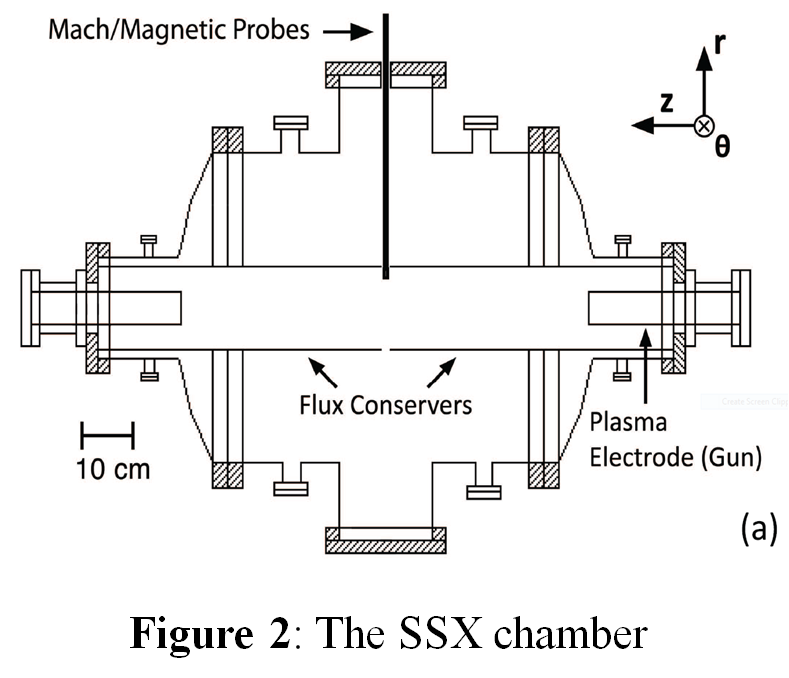
\includegraphics[width=8.5cm]{chamber.png}}
\caption{\label{fig:chamber} Cross-section of SSX chamber in MHD wind-tunnel configuration}
\end{figure}

\section{Results}

\begin{figure}[!htbp]
\centerline{
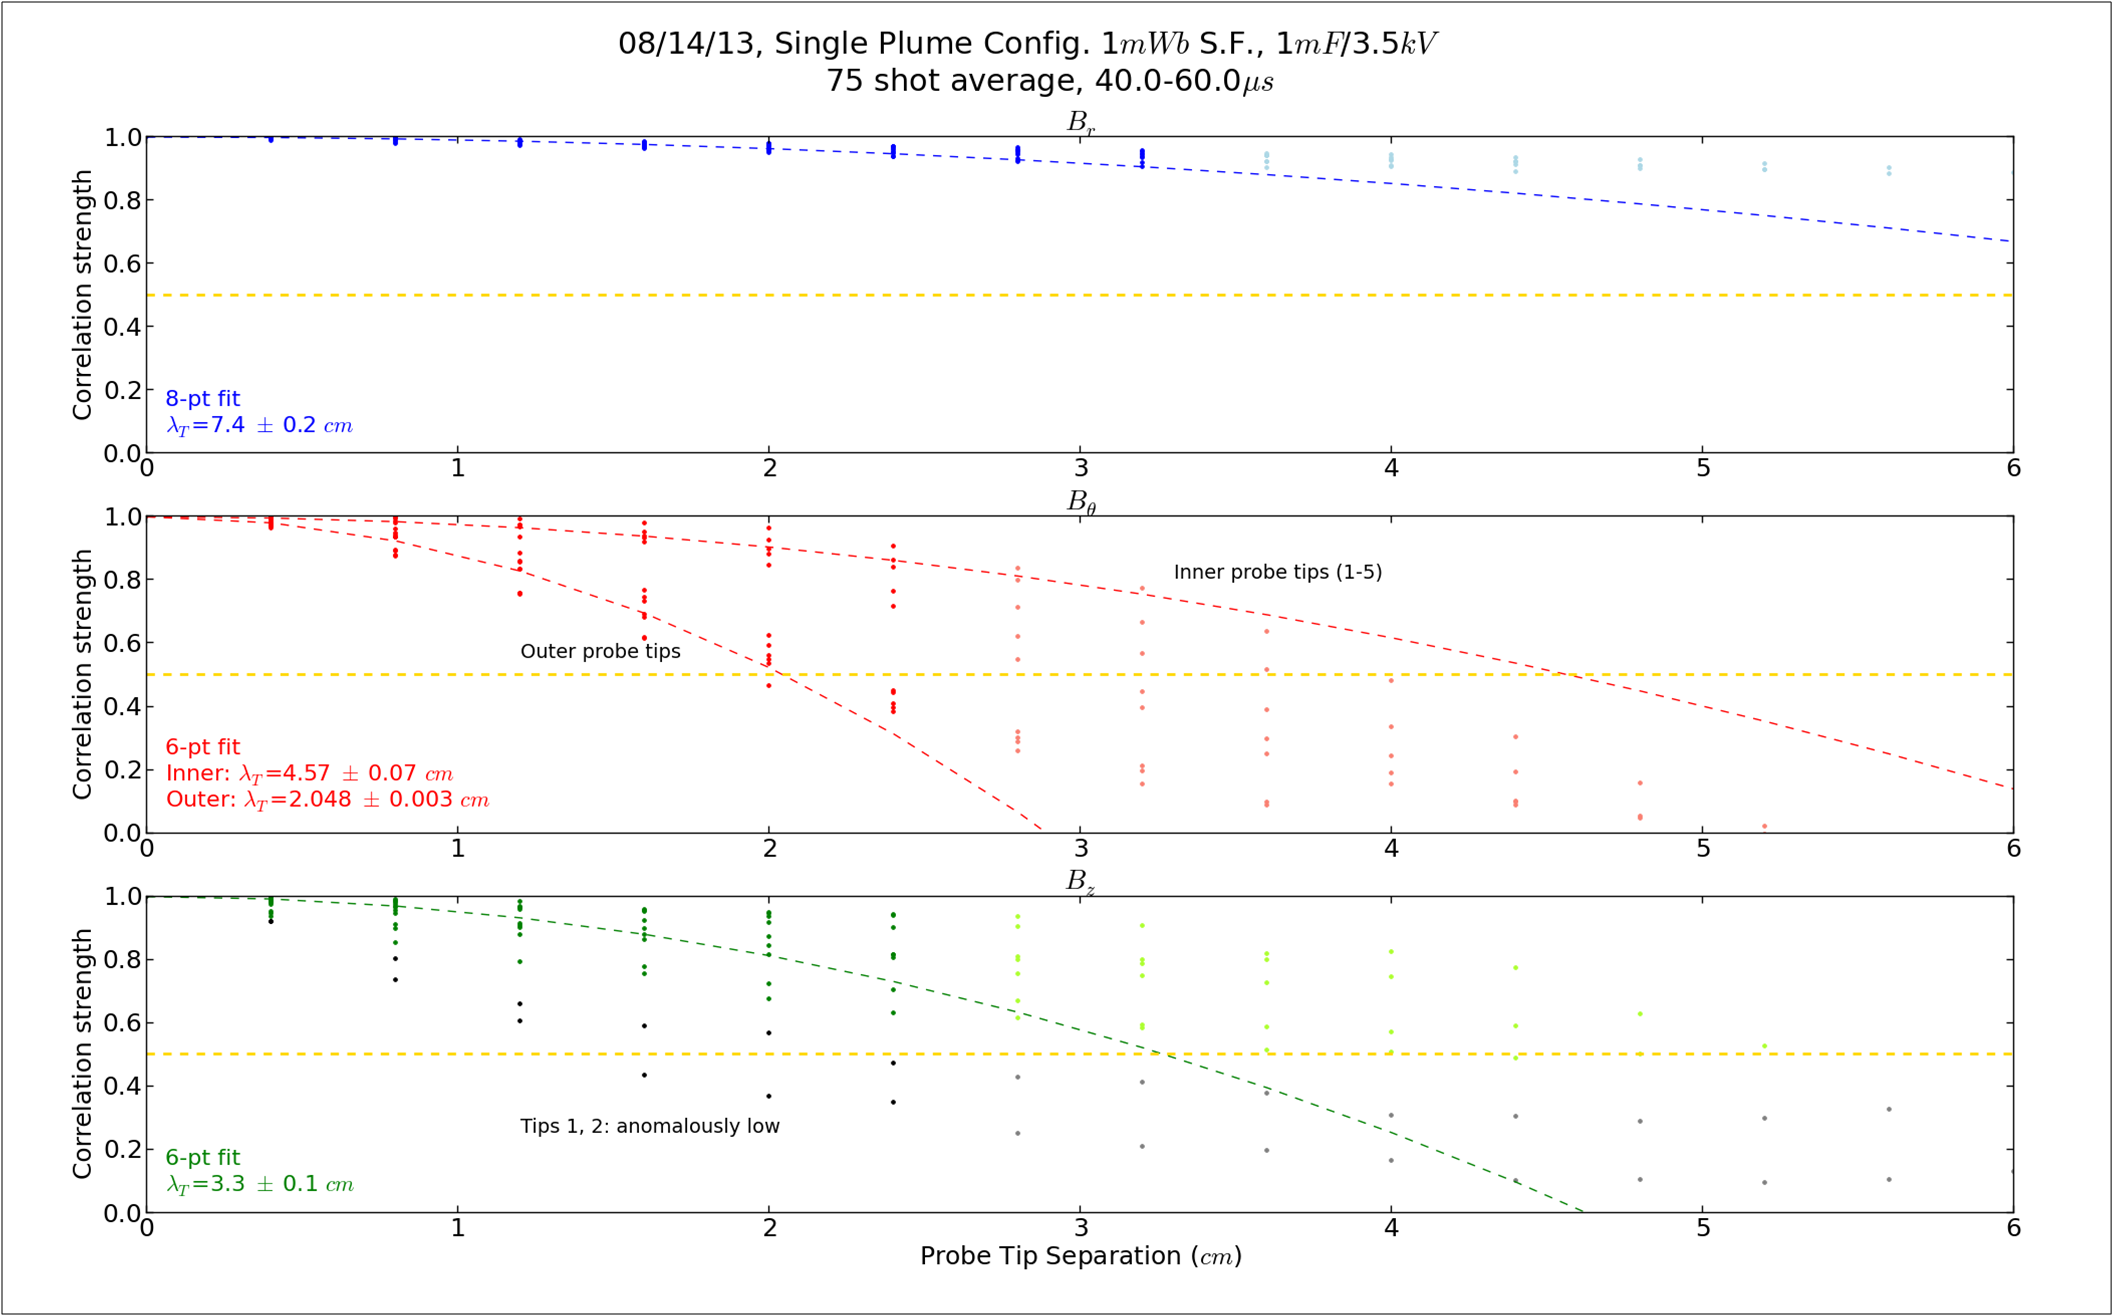
\includegraphics[width=8.5cm]{BrBtBz_correlations.png}}
\caption{\label{fig:BrBtBz_correlations} Correlations Functions}
\end{figure}

\begin{figure}[!htbp]
\centerline{
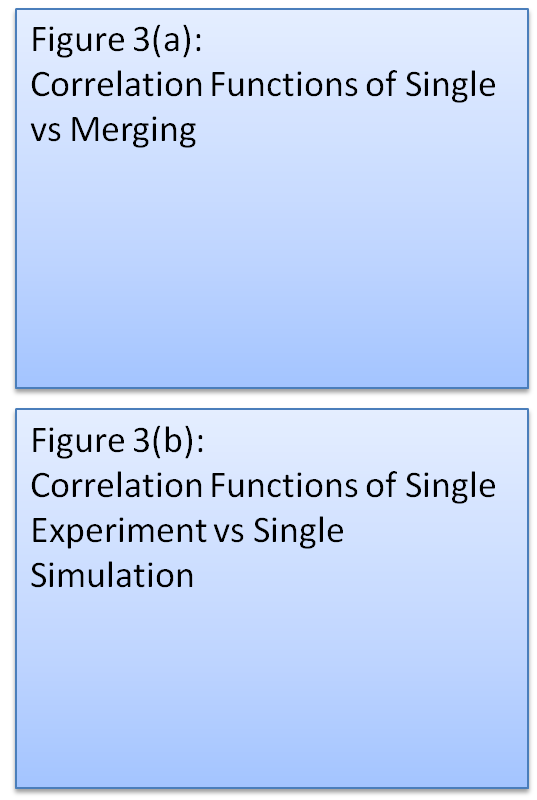
\includegraphics[width=8.5cm]{figure3_placeholder.png}}
\caption{\label{fig:figure3_placeholder} (a) Single vs Merging. (b) Expt vs Sim.}
\end{figure}

\begin{figure}[!htbp]
\centerline{
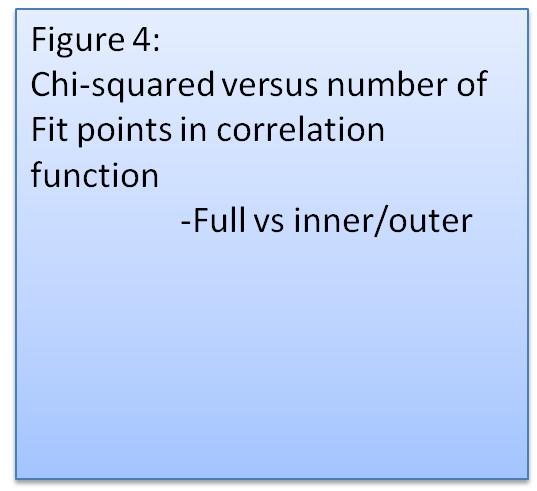
\includegraphics[width=8.5cm]{figure4_placeholder.png}}
\caption{\label{fig:figure4_placeholder} $Chi^{2}/n$ of parabolic fit versus n.}
\end{figure}

\begin{table}
\caption{\label{tab:Rms}Comparison of measured/computed Taylor Microscale and magnetic Reynolds numbers for various cases.}
\begin{tabular}{|l|l|l|l|l|l|}
\hline
Condition&$\lambda_{CS}$&$\lambda_{T}$&$R_{m}$ w/Radius&$R_{m}$ w/Int. Scale&$R_{m}$ Computed\\
\hline
Single-Outer&1&1&1&1&1\\
Single-Inner&1&1&1&1&1\\
Merging&1&1&1&1&1\\
Simulation&1&1&1&1&1\\
\hline
\end{tabular}
\end{table}

% ----------------------------------------------------------------
\section*{Acknowledgements}
%  We gratefully acknowledge many useful discussions with William Matthaeus. This work has been funded by the US DoE Experimental Plasma Research program and the National Science Foundation.  The simulations were performed using the advanced computing resources (Cray XC30 Edison system) at the National Energy Research Scientific Computing Center.
% ----------------------------------------------------------------
\section*{References}
\begin{thebibliography}{99}

\bibitem{Belmabrouk98}
Belmabrouk, H., and M. Michard (1998), Taylor length scale measurement
by laser Doppler velocimetry, Exp. Fluids, 25, 69Ð76.

\bibitem{Matthaeus05}
Matthaeus, W. H. and Dasso, S. and Weygand, J. M. and Milano, L. J. and Smith, C. W. and Kivelson, M. G., Phys. Rev. Lett. 95, 231101 (2005) Spatial Correlation of Solar-Wind Turbulence from Two-Point Measurements

\bibitem{Weygand07}
Weygand, J. M., Matthaeus, W. H., Dasso, S., Kivelson, M. G.,
and Walker, R. J. (2007), J. Geophys. Res., 112, A10201.

\bibitem{Weygand09}
Weygand, J. M., Matthaeus, W. H., Dasso, S., Kivelson, M. G.,
Kristler, L. M., and Mouikis, C. (2009), J. Geophys. Res., 114,
A07213.

\bibitem{Weygand10}
Weygand, J. M., Matthaeus, W. H., El-Alaoui, M., Dasso, S., and
Kivelson, M. G. (2010), J. Geophys. Res., textit115, A12250.

\bibitem{Weygand11}
Weygand, J. M., Matthaeus, W. H., Dasso, S., and Kivelson, M.
G. (2011), J. Geophys. Res., 116, A08120.

\bibitem{Matthaeus08}
Matthaeus W. H., Weygand, J. M., Chuychai, P., Dasso, S.,
Smith, C. W., and Kivelson, M. (2008), Astrophys. J., 678,
L141.

\bibitem{frisch95}Frisch, U. 1995, {\it Turbulence} (Cambridge: Cambridge Univ. Press)

%\bibitem{sorrisovalvo99}Sorriso-Valvo, L. {\it et al.} Geophys. Res. Lett. {\bf 26}, 1801–1804 (1999).

%\bibitem{wan12}Wan, M. {\it et al.} ApJ. {\bf 744} 177 (2012).

%\bibitem{sorrisovalvo01}Sorriso-Valvo, L. {\it et al.} Planet. Space Sci. {\bf 49}, 1193–1200 (2001).

%\bibitem{marrelli05}Marrelli, L. {\it et al.} Phys. Plasmas. {\bf 12}, 030701 (2005).

%\bibitem{Greco08}A. Greco, P. Chuychai, W. H. Matthaeus, S. Servidio and P. Dmitruk, Intermittent MHD structures and classical discontinuities, Geophys. Res. Lett. {\bf 35}, L19111 (2008).

%\bibitem{Greco09}Greco, A., Matthaeus, W. H., Servidio, S., Chuychai, P., and Dmitruk, P.: Statistical Analysis of Discontinuities in Solar Wind ACE Data and Comparison with Intermittent MHD Turbulence, ApJ {\bf 691}, L111 (2009).

%\bibitem{Wan09}Wan, M., Oughton, S., Servidio, S., and Matthaeus, W. H.: Generation of non-Gaussian statistics and coherent structures in ideal magnetohydrodynamics, Phys. Plasmas {\bf 16}, 080703 (2009).

%\bibitem{Servidio11b}Servidio, S. {\it et al}, J. Geophys. Res. {\bf 116}, A09102 (2011).

%\bibitem{Gray13} T. Gray, M. R. Brown, and D. Dandurand. Phys. Rev. Lett. {\bf 110}, 085002 (2013). 

%\bibitem{schaffner14} D.A. Schaffner {\it et al.} Turbulence analysis of an experimental flux rope plasma. Submitted to Plas. Phys. Cont. Fusion. (2014).

%\bibitem{Taylor86} J. B. Taylor, Rev. Mod. Phys. {\bf 58}, 741 (1986).

%\bibitem{Matthaeus80} W.H. Matthaeus and D. Montgomery, Ann. N.Y. Acad. Sci. {\bf 357}, 203 (1980).

%\bibitem{torrence98}C. Torrence, G.P. Compo, A practical guide to wavelet analysis. Bull. Am. Meteorol. Soc. {\bf 79}, 6178 (1998).

%\bibitem{clauset09}A. Clauset, C. Rohilla Shalizi, M.E.J. Newman, Power-law distributions in empirical data, SIAM Rev. {\bf 51}, 661703 (2009).

%\bibitem{wan12}M. Wan, K. T. Osman, W. H. Matthaeus, and S. Oughton, Investigation of intermittency in magnetohydrodynamics and solar wind turbulence: scale-dependent kurtosis, ApJ {\bf 744}, 171 (2012).

%\bibitem{Gray10}T. Gray, V. S. Lukin, M. R. Brown, C. D. Cothran, Three-dimensional reconnection and relaxation of merging spheromak plasmas, Phys. Plasmas {\bf 17}, 102106 (2010).

%\bibitem{goldstein94}Goldstein, M.L., Roberts, D.A. and Fitch, C.A. Jour. Geo. Res. {\bf 99} 11519-11538 (1994).

%\bibitem{ji95}Ji, H., Prager, S.C. and Sarff, J.S. Phys. Rev. Lett. {\bf 74} 2945 (1995).

%\bibitem{telloni12}Telloini, D. {\it et al.}. ApJ. {\bf 751} 19 (2012).

%\bibitem{matthaeusVelli11}Matthaeus, W.H. and Velli, M. Space Sci. Rev. {\bf 160} 145-168 (2011).

%\bibitem{greco12}A. Greco {\it et al.} ApJ. {\bf 749} 105 (2012).

\end{thebibliography}

\end{document}

